% Template GRASS newsletter - Article Language: Latex LA This
% project aims to define a settlement's use of, and impact on, their
% surrounding landscape.

% Head

\title{LA} \subtitle{Identifying Landuse Catchments for 
ancient settlements.}

\author{by Jason Jorgenson and Tim Sutton}

\maketitle

\section{Introduction} \label{sec:Introduction}

This paper describes a software application we are developing that automates
the process of computing landuse requirements for any settlement of people.
The examples used throughout are of the archaeological site Shuna (see Figure
\ref{fig:shunaGoogleEarth}) in the Jordan Valley.
The Jordan Valley is found in the Southern Levant, which is
a name commonly used to refer to the geographic region broadly described as
modern-day Israel, Palestine and Jordan, between the Dead Sea and Lake
Tiberias.

\begin{figure}[htbp] %Location
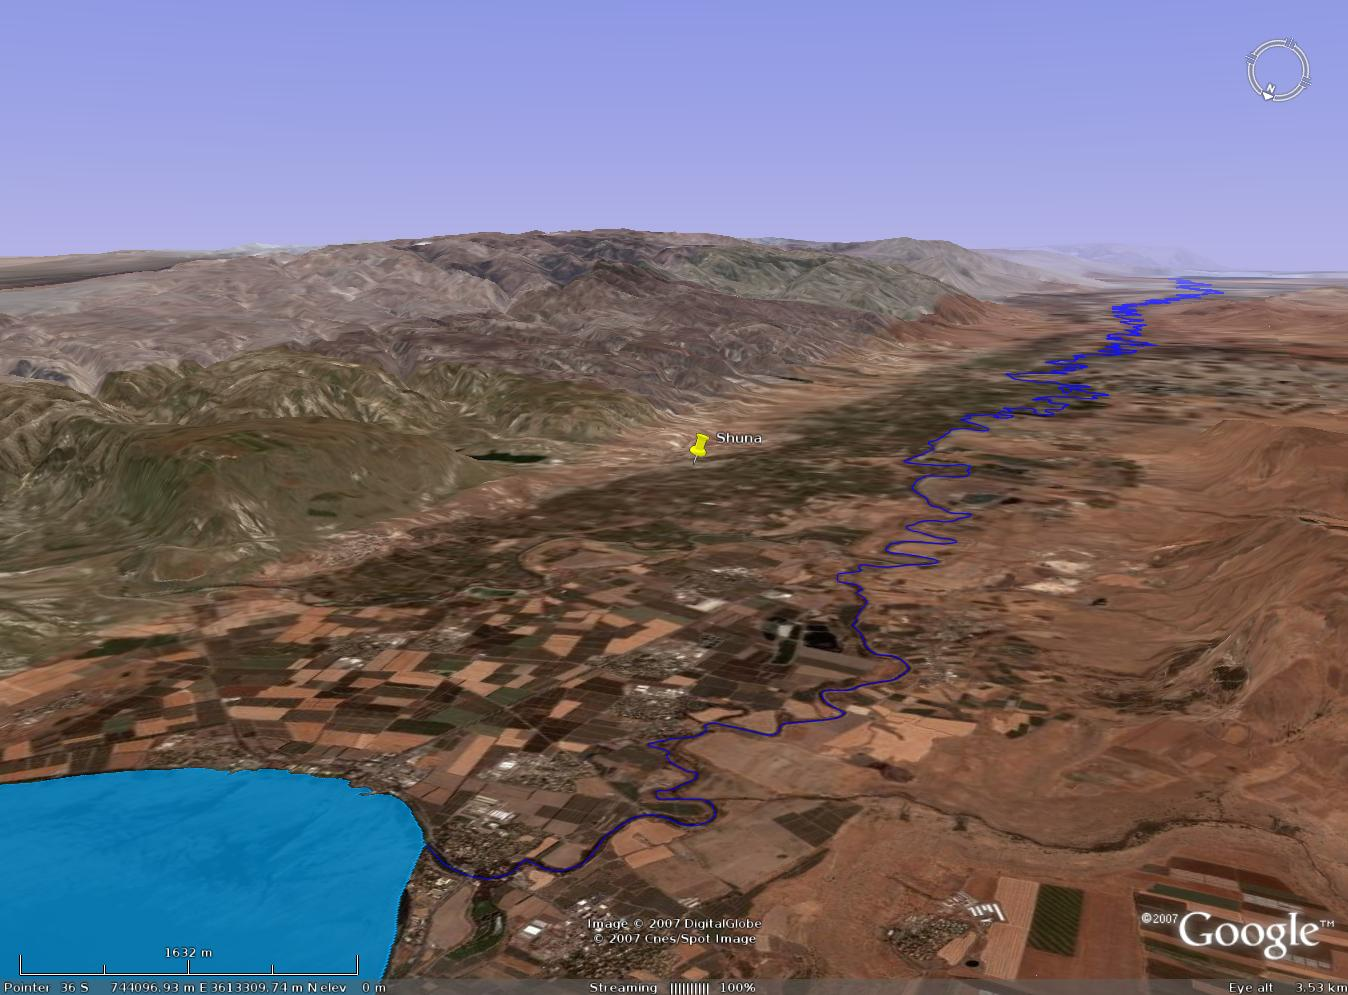
\includegraphics[scale=0.17]{./images/ShunaGoogleEarth3D.jpg}
% img42.jpg: 800x600 pixel, 72dpi, 28.22x21.17 cm, bb=0 0 800 600
\label{fig:shunaGoogleEarth} \caption{Looking South-South-East from Lake
Tiberias Down the Jordan Valley towards Shuna.} \end{figure}

We describe how the application logic for Landuse Analyst (LA) was prototyped as
a
BASH shell script calling various GRASS utilities, and then developed into a
more flexible application with a graphical user interface.

\section{Background} \label{sec:Background} For an archaeologist, understanding
the relationship that existed between people in the past and their landscape is
very important.  People throughout time have relied on various plants and
animals, wild or domestic, to provide them with the food they require to
survive.  Regardless of the period in time being examined, a relationship
exists between people and the space which they occupy.  A better understanding
of this relationship can help to more confidently theorise about a range of
issues in the reconstruction of past societies.  Imagine, for example, the
relationship that nomadic hunter gatherers had with the land, and then compare
that to  an artisan living in a settlement of several thousand people.  We can
piece together clues revealed through a combination of archaeological surveys,
ethnoarchaeology, written records, oral traditions, and excavations. The
insight gained from these clues can offer a more concrete understanding of the
relationship people had with their landscapes, allowing archaeologists to
better understand topics such as social and economic organisation\footnote{In
one sense, economic organisation can be thought of as the strategy used to
collect and distribute resources.  In modern societies, urban centres rely upon
the surplus production of agricultural commodities provided by farmers in the
countryside.  This reliance necessitates a certain level of organisation
between rural and urban people.  By applying this same logic in historical
contexts, we can infer landuse patterns .}, as well as short and long term
impacts communities might have had on the landscape.  An understanding of long
term impacts of ancient humans on their landscape can be useful for modern day
researchers by, for example, providing insight into the potential environmental
impact of
current human activities.

\section{Evidence} \label{sec:Evidence} By examining seeds, bones, and other
items found at archaeological sites, archaeologists are able to determine 
dietary habits. From the relative quantities found estimates can be made of the
importance each food source would have had in the diet.  Specific agricultural
practices
can be detected in the archaeological record in a number of ways.  If the scale
of production is known, crop selection, for example, can help indicate whether
crops were being cultivated for subsistence use or for more commercial
purposes\footnote{Sometimes, written accounts exist which can help to
piece this together.}.  If there is evidence of surplus production of any
particular crop or animal, this can be a possible indication that it was being
grown commercially.  Other possible inferences include taxation, storage,
redistribution, indications of intensified farming, and craft specialisation,
all of which can indicate increased economic complexity.  Through careful
study, a better understanding of the land use habits and patterns of these
populations can unlock many interesting facets of the culture and lifestyle of
these peoples.

\section{Process for computing landuse requirements} \label{sec:EarlyAttempts} 

In order to learn more about how people interacted with their land, it is very
helpful to determine an approximate area of land needed to support settlement
populations and it's likely distribution.  In order to do this, it is necessary
to first know how much land would have been needed to produce enough food to
sustain the settlement.  A three step process is used to calculate the amount of
land a settlement would have required based on it's population and diet
make-up.  

\begin{enumerate}
 \item Calculating Calorie Targets
 \item Calculating Production Targets
 \item Calculating Area Targets
\end{enumerate}
These are discussed in more detail later.

Once an area target is known, the land surrounding the
site must be classified as either suitable or unsuitable for each crop sown and
each type of animal being raised.  Lastly, the area target from the first step
can be used to query the land suitability classification map for that area of
land surrounding the site.

From a GIS point of view, one of the greatest challenges of this project was
developing a method for finding the outer extent (or boundary), within which
the combined area of suitable land satisfies the target area.  The usable land
surrounding a settlement is almost certainly not going to contiguous, but
rather be comprised of multiple, irregularly shaped polygons. A further
complication is the fact that some of the irregularly shaped polygons may
be bisected one or more times by the 'boundary line'.  

In late 2006, a BASH script was created running in a GRASS shell.

This script found a specific area of classified, suitable land surrounding a
point (Fig.\\ref{fig:euclideanResults})  by starting at a point and moving
outwards in a circle five meters at a time, checking each time to see if there
was enough suitable land contained with the perimeter.  As soon as it was equal
to or greater than the target area, the loop was ended, and the solution was
deemed found.

\section{Moving to a graphical user interface} \label{GUI} 
 
The complexity of the animal and crop modelling made using BASH scripts very
awkward.  While the BASH scripting approach worked well for a proof of concept,
the implementation included a large number of hard coded variables and the
solution 
did not provide a flexible environment for experimentation. For example, adding,
removing or even 
editing different types of crops and animals to the analysis required heavy
modifications 
to the BASH script.  The BASH script approach approach also had poor reporting
capabilities and offered little 'hand holding' to the user as the analysis was 
carried out.

Consequently we embarked on the development of a Graphical User Interface (GUI)
based 
application (see Fig. \ref{fig:la544}), written in C++ and Qt4. This programming
environment decision was largely 
motivated by a desire to capitalise on existing code bases from openModeller
\footnote{openModeller is available at
\url{http://openmodeller.sourceforge.net/}} 
and Quantum GIS (QGIS)\footnote{QGIS is available at \url{http://qgis.org}}.  
For invoking GRASS tools we opted to use QProcess to launch GRASS commands in 
their own process and then implemented application logic to parse the results
of 
each command from stdout.

\begin{figure}[htbp] %Proof of Concept
  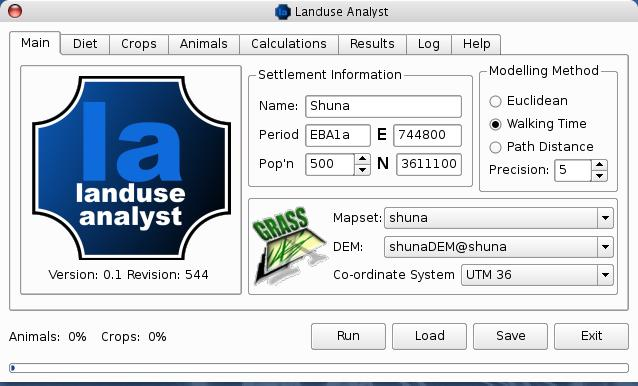
\includegraphics[scale=0.36]{./images/LanduseAnalyst544.jpg}
   % img42.jpg: 800x600 pixel, 72dpi, 28.22x21.17 cm, bb=0 0 800 600
   \label{fig:la544} \caption{LA's primary interface}
   \end{figure}


\section{Analytical functionality} \label{sec:Analytical Functionality}

LA includes various routines for calculating the amount of land 
the settlement needs.  Briefly, these can outlined as follows:

  \begin{enumerate} 
  \item Breaking down the basic diet of the community into specific crops and
  animals being used for nourishment.  Each individual crop and animal needs to
  be expressed as a percentage of the peoples' diet.  This is estimated using
  proportions based on archaeological evidence such as faunal and
  paleobotanical remains discovered from excavations.  
  \item Calculating  calorie targets for the crops and animals identified above.
 
  \item Calculating production targets which fulfil the calorie targets.
  Production targets are calculated in kilograms, and take into account factors
such as 
  calories per kilogram of produce, and what percentage of an animals weight is
  usable as food.  
  \item Calculating land area targets needed to satisfy the
  production targets.  Each crop and animal is allocated a specific area
  target.  
  \item Carrying out a spatial analysis of the land surrounding the settlement
to
  find land suitable for each crop and animal that satisfies the area targets.  
  \end{enumerate}

The details of how these targets are determined are a major part of Landuse
Analyst, but largely beyond the scope of this article.  A brief overview
follows.

\subsection{Step 1: Determine calorie targets}
  \index{LA!Calorie targets}
  Calorie targets are the first level of calculations done by LA.  Calorie
targets are determined 
through a number of steps (see Fig. \ref{fig:dietDiagram}), which are as
follows.


\begin{figure}[ht] %dietDiagram
 \centering
 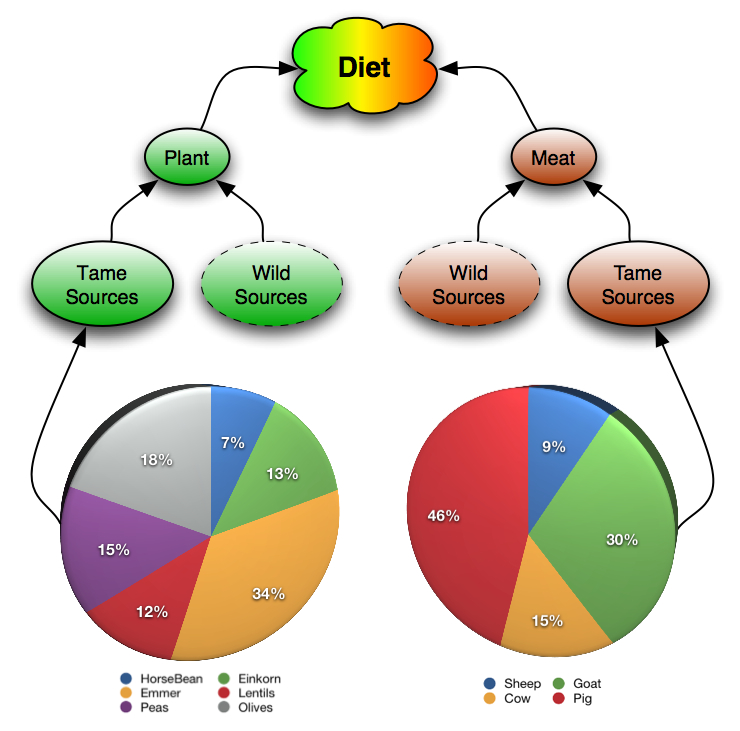
\includegraphics[scale=.32]{./images/dietDiagram.jpg}
 % dietDiagram.jpg: 740x731 pixel, 72dpi, 26.10x25.78 cm, bb=0 0 740 731
 \textit{\caption{\label{fig:dietDiagram}Conceptual diagram of a settlement's
diet composition.}}
\end{figure}

\begin{figure}[ht] %dietMeatDiagram
 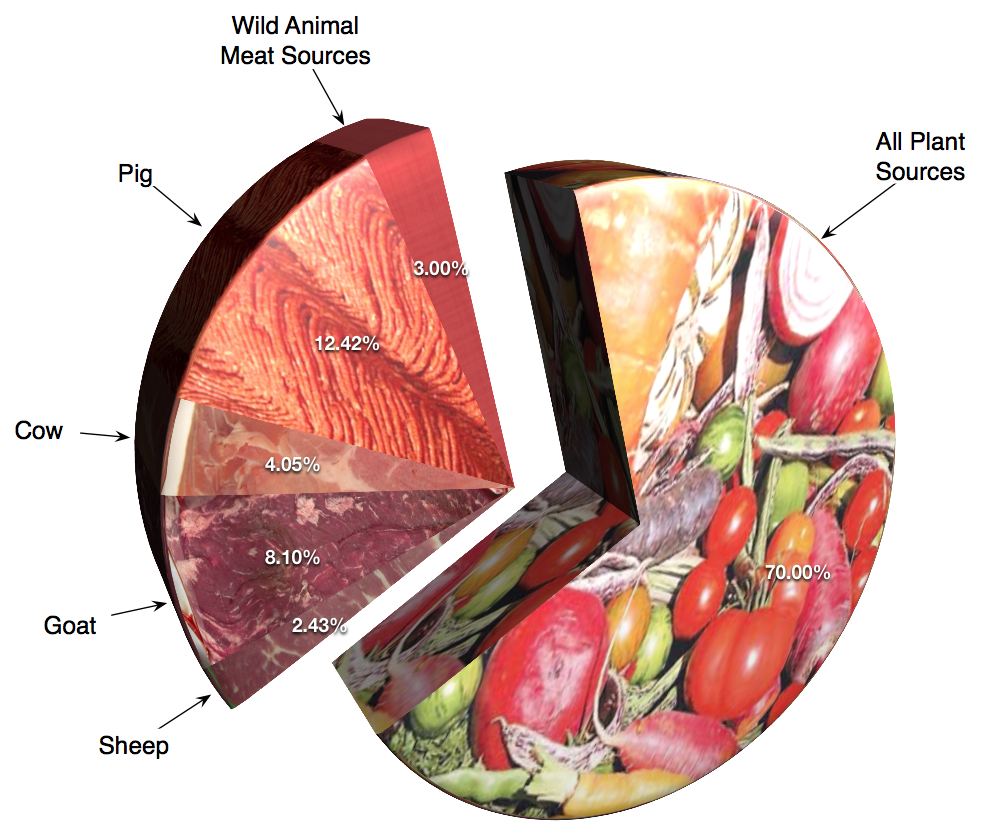
\includegraphics[scale=.23]{./images/fancyDietMeat.jpg}
 % dietDiagram.jpg: 740x731 pixel, 72dpi, 26.10x25.78 cm, bb=0 0 740 731
 \textit{\caption[Plant Portion of Diet]{\label{fig:dietMeatDiagram}Conceptual
diagram of meat component of diet.}}

\end{figure}

\begin{figure}[ht] %dietCropDiagram
 \centering
 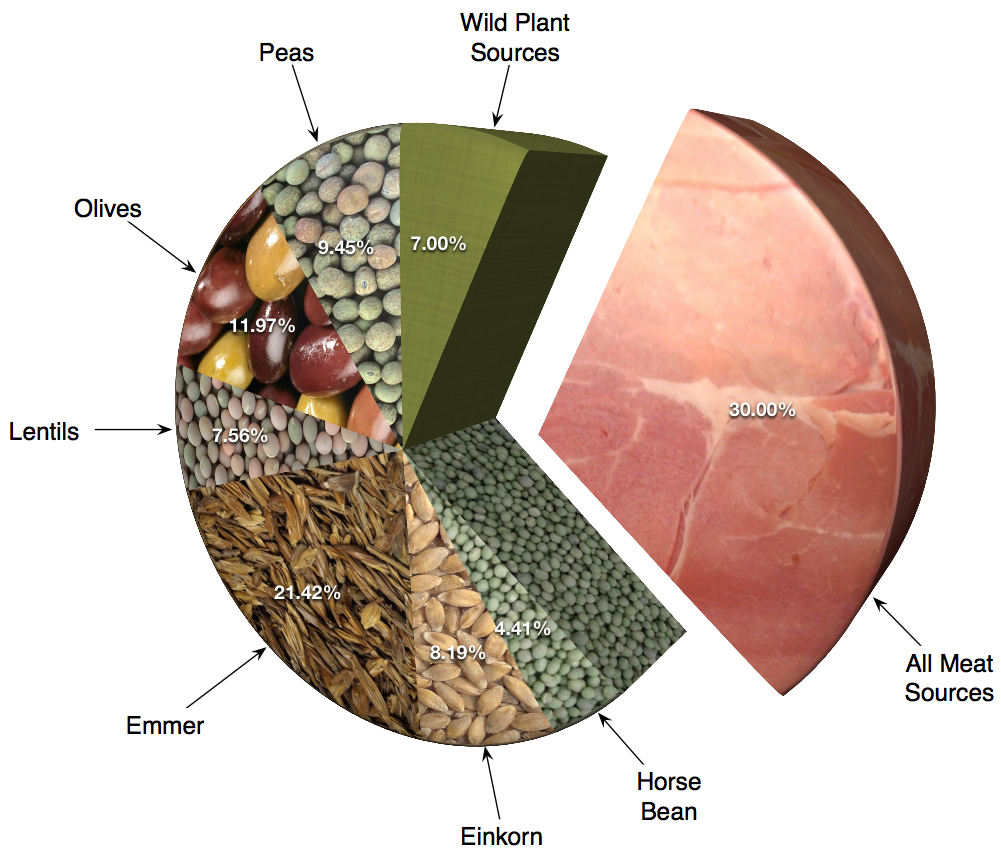
\includegraphics[scale=.2]{./images/dietFancyCrops.jpg}
 \textit{\caption[Plant Portion of Diet]{\label{fig:dietCropDiagram}Conceptual
 diagram of the plant component of diet.  Note that the input figures for
 percent of diet were: \textbf{HorseBean} $7\%$, \textbf{Einkorn} $13\%$,
 \textbf{Emmer} $34\%$, \textbf{Lentils} $12\%$, \textbf{Peas} $15\%$,
 \textbf{Olives}\ $18\%$.  These numbers translate to those shown above after
 processing as in Fig. \ref{fig:dietDiagram}.}}
\end{figure}

    \begin{enumerate}
      \item \textbf{\textit{Basic Information}} - The user supplies LA with the
      population of the settlement, as well as the average daily calorific
      requirements of an average member of the population.  By multiplying
      these figures together, the total number of calories required for the
      settlement is calculated (see Fig. \ref{fig:LADiet}).

      \item \textbf{\textit{Primary Dietary Components}} - This step works on
      the principle that calories can come from only two fundamental sources:
      plants and animals.  By adjusting a slider right or left, this overall
      ratio is set.  To explain how this works, let's say that the yearly
      calorific requirement for a settlement is $1,000,000$.  If the slider is
      set to show $70\%$ Plants and $30\%$ meat, this would mean that LA will
      calculate the number of calories that need to come from Plants as
      $700,000$ and those that need to be supplied by meat as $300,000$.

      \item \textbf{\textit{Detailed Dietary Components}} - At this step, the
      process gets split into two sections.  One section is for the Plant
      portion of the diet, and the other is for the Meat portion.  Again, the
      calculations are done based on values which are set by a slider that
      indicates what percentage of the plants or animals come from domestic
      sources.  To illustrate this, we will continue using the figures above of
      $700,000$ for plants and $300,000$ for animals.  If the slider on the
      plant side is set to $90\%$ Tame\footnote{The word tame was used purely
      for aesthetic purposes in the design of the input form of LA} then the
        number of calories that need to be supplied by domestic plants (crops)
        would be $700 \cdot 90\%$ or $630,000$ calories.  

      \item \textbf{\textit{Crop/Animal Contributions}} - The final step is
      easy to understand, but is not done in the Diet section of the program.
      Rather, it is calculated using values that are supplied as parameters for
      each individual crop and animal.  This parameter is set with a spin-box
      in the Parameter Manager form.  This value tells LA that this individual
      animal or crop comprises the indicated percentage of the calories being
      supplied by tame sources, which is the value from the previous step. As
      an example, if peas are defined as a crop, and the percentage of diet
      setting in Wheat's Parameters is set to $15.00\%$ then using the values
      from the previous step, LA calculates that Peas must provide $630,000
      \cdot 15.00\%$ or $94,500$ calories.  This also means that Peas represent
      $15\%\cdot90\%\cdot70\%=9.45\%$ of the overall diet.  Remember that the
      $15\%$ is a portion of the \textit{tame crop} part of the diet! ( See
      Fig. \ref{fig:dietCropDiagram} and Fig. \ref{fig:dietMeatDiagram}).  The
      exact same thing happens with meat.
    \end{enumerate}

\begin{figure}[htbp]
  \label{fig:LADiet}%LADiet
    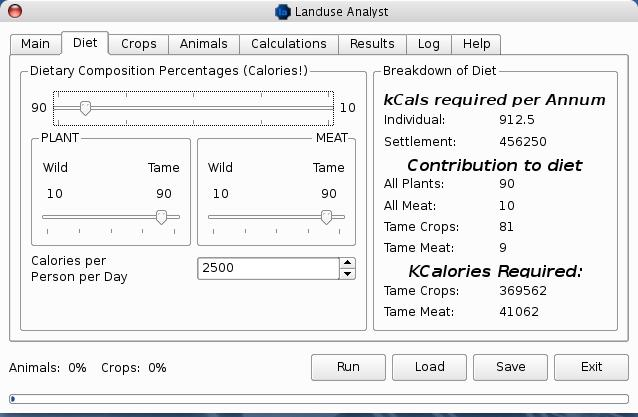
\includegraphics[scale=.355]{./images/LanduseAnalystDiet545.jpg}
    % LanduseAnalystDiet545.jpg: 638x417 pixel, 762dpi, 2.13x1.39 cm, bb=0 0 60
39
  \caption{ Diet Tab, LA}
\end{figure}

\subsection{Step 2: Determine production targets}
  \index{LA!Production Targets}
  Production targets are measures of weight, and represent how many Kg of each
  crop and animal must be produced to satisfy the calorie targets calculated
  above.  Because crops and animals need to be treated somewhat differently at
  this stage, they will be dealt with in separate sections, beginning with Crops
  as they are most easily explained.

  \subsubsection{Crops}
The user must supply a food value of each crop.  Using the calorie targets and
the user supplied food value, the model calculates the production target
necessary to meet these needs.

  \subsubsection{Animals}
When animals get slaughtered, and only part of their carcasses are usable as
food.  This usable part of their live weight is supplied by the user when they
define the animal in the Animal Manager form, expressed as the percentage of
their live weight which is usable as food.

\subsection{Step 3: Determine area targets}
\index{LA!Area Targets}
Once production targets are calculated, it is possible to calculate area
targets for each crop and animal by looking at yield values for plants, and
grazing requirements for animals.  As with Production Targets, Area Targets are
quite simple to compute for crops, but get very complicated for animals.

  \section{Crops}
    A list of all crops that have been defined is found when the Crops tab is
    clicked (Fig. \ref{fig:crop}).  Note that the user has the choice of
    selecting it for inclusion in the model, as well as being able to select
    different parameters from a drop-down list.  To the right of the drop down
    list is the crop's contribution to the tame plant portion of the diet using
    the currently selected parameter.  The total of these percentages must be
    equal to $100\%$ before the model will run, and the current total is always
    visible in the bottom left hand corner of the form.

    \begin{figure}[htbp]
        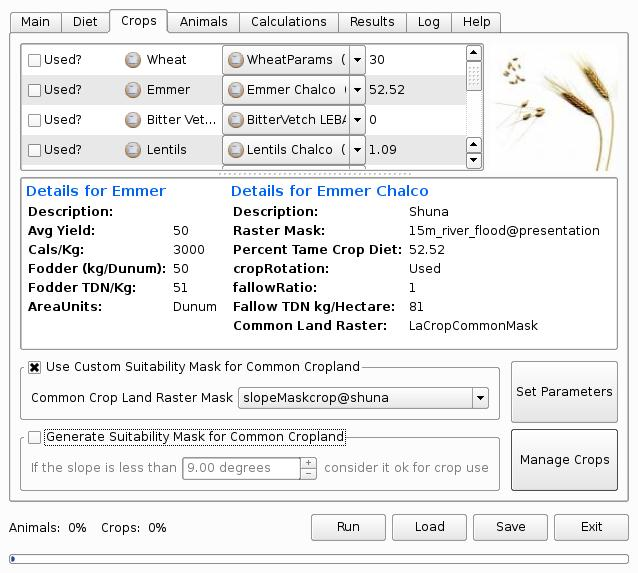
\includegraphics[scale=.366]{./images/LanduseAnalystCrops546.jpg}
      \label{fig:crop} \caption{Crops Tab, LA Version 0.1 Revision 544}
    \end{figure}
    
  \textbf{Crop rotation}\index{LA!Crop Rotation} affects the area target
  directly, so a few points about it need to be mentioned.  Quite simply, LA
  treats crop rotation as a ratio of sown land to fallow land.  If a ratio of
  $1:1.00$ is used, this means that the practise was to sow their land every
  other year and leave last years cropland fallow (More complicated crop
  rotations are possible in LA, and the process of setting this up are
  explained in more detail in the Help section of the program itself).  The
  crop rotation data is entered as a crop parameter in the Crop Parameter form
  (See Fig. \ref{fig:cropParameters} ).
    \begin{figure}[htbp] %crop parameters
        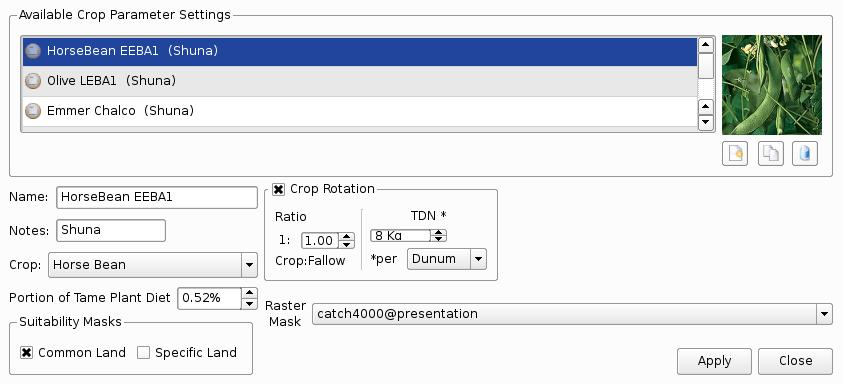
\includegraphics[scale=.28]{./images/cropParameters.jpg}
        % cropParameters.jpg: 842x384 pixel, 762dpi, 2.81x1.28 cm, bb=0 0 80 36
      \caption[Crop Parameters]{\label{fig:cropParameters}\textit{Crop
Parameters form for setting the particulars of the crop.}}
    \end{figure}


\section{Animals}
Animals are difficult to calculate area targets for because their land
requirements are largely based on their numbers, and a herd of adult
females large enough to sustain a steady supply of offspring with numbers
enough to keep the production targets met has to be added into the equation as
well.  In addition, animals can graze fallow crop land, eat fodder from
the crops being grown, and graze other types of land.  LA takes these
interactions into account in its computations.
Herd Size determination is perhaps the single most difficult calculation that
LA performs.  Added to the complexity of this is the problem that different
animals have different dietary requirements, and even further, even if they
are the same, they require different amounts of feed depending on things like
whether they are pregnant or lactating, and what the weather conditions are
like.  Again, to further complicate this issue, not all land that can be
grazed has the same food value to the animals.

With the exception of weather conditions, LA addresses these issues.  One of
the first things a user must do when using Landuse Analust is to define all
of the crops and animals that the settlement used.  During this process the
users provides information about aspects including (for animals) information
relating to their dietary requirements, their reproduction cycle, and their
grazing preferences.  


      \label{TDN}
      \index{TDN}
      \index{Total Digestable Nutrients}
    \textbf{TDN} is an acronym for \textbf{T}otal \textbf{D}igestable
    \textbf{N}utrients, and is a commonly used term among ranchers to describe
    the quality of the feed available to their animals, and is expressed as a
    measure of weight.  TDN can be used for any grazing animal, and since the
purpose of LA is to identify the land which a settlement was using for food
production, this is all we need.


\section{Defining Crops}\index{Crops!Defining}Every crop has unique
characteristics, and Landuse Analyst splits these defining qualities into two
main areas.
  \subsection{Defining the Plants}\index{Crops!Plant Definition}First, there is
the plant itself, which has seven input fields (see Fig. \ref{fig:cropManager} .
    \begin{enumerate}
      \item \textbf{\textit{Name}}

      \item \textbf{\textit{Notes}}

      \item \textbf{\textit{Yield}}

      \item \textbf{\textit{Food Value}}

      \item \textbf{\textit{Fodder}}

      \item \textbf{\textit{TDN}}

      \item \textbf{\textit{Area Units}}
    \end{enumerate}

      \begin{figure}[htbp]
        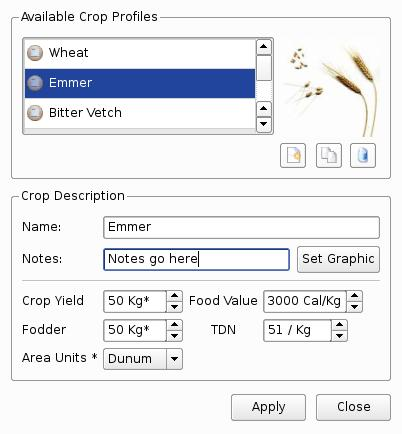
\includegraphics[scale=.6]{./images/cropManager.jpg}
        % cropManager.jpg: 402x434 pixel, 762dpi, 1.34x1.45 cm, bb=0 0 38 41
      \label{fig:cropManager} \caption{Crop Manager}
    \end{figure}


  \subsection{Crop Parameters}
  \label{cropParameters}
  Once you have defined the plants that are being grown as crops, Landuse
Analyst needs to know the specifics of how each crop is being grown, as well as
what portion of the settlement's diet it provides (see Fig.
\ref{fig:cropParameters}).  It must also
know what land is capable of growing each crop by selecting either Common or
Specific Land Suitability masks (keeping in mind that if Specific Land is
selected, the Raster Mask must be selected from the drop down list).  The two
major entries, however, involve \textit{crop rotation} and the selection of
\textit{suitability masks}.

    \subsection{Crop Rotation}
    \label{cropRotation}
    A common farming technique still used widely even today is the practise of
resting your cropland every growing season or so.  This is called \textit{crop
rotation} and is critical to the process of determining how much land is
required for food production, as it can more than double the necessary area. 
Take a simple scenario where a farmer sows ten hectares of wheat, and leaves
another ten hectares \textit{fallow}\footnote{fallow is a term used to describe
land that is 'resting' from growing a crop, having previously done so.}.  The
following year, he sows the ten hectares of 'rested' fallow land, and leaves
last year's cropland to rest (as fallow).  This type of rotation, sowing ten
hectares and fallowing ten hectares, can be described with a ratio of
\textbf{\textit{Sown Land}} to \textbf{\textit{Fallow Land}} or in this case,
$1:1.00$ .  Note that two decimal places are used when describing the portion
for fallow land.  This is to accommodate more complex crop rotation regimes. 
Such a regime might be sowing ten hectares of wheat in year one, then the same
ten hectares to lentils in year two, and fallowing the same in year three.  In
order to maintain the production of lentils and wheat using this rotation, the
farmer needs ten hectares of cropland for wheat, another ten hectares for
lentils, and still have enough fallow to rest the land in the rotation every
third year.  In any given year, between the three parcels of land, there are two
parcels of land being sown, and one parcel of land in fallow.  This is a ratio
of $2:1.00$ .  This needs to be expressed as a $1:x$ ratio however, so we must
multiply both by the reciprocal of the value for crop.  In this case, the crop's
value is $2$, and the reciprocal of $2$ is $\frac{1}{2}$ so we end up with:
$\frac{2}{2}:\frac{1.00}{2} = 1:0.50$.

    Another important aspect of defining crop rotation concerns animals.  It is
possible for animals to graze the fallow land, which will reduce the amount of
grazing land otherwise required to sustain the animals.  In order to know how
much contribution the fallow land makes, it is necessary to know the food value
of the fallow land.  Using the ratio of crop land to fallow land along with the
food value of the fallow land allows Landuse Analyst to accurately adjust the
grazing land requirements for the animal herds.  How this is done is explained
in detail in the following section.

\section{Defining Animals}
  \label{definingAnimals}
Animals present several challenges that plants do not.  For starters, a certain
number of females must be kept solely as breeding stock, and this number must be
calculated based production requirements.  Secondly, the possibility exists that
par of the animals' diet was from either straw/chaff left over from harvesting
crops, or directly from harvested grain.  In the case of grain being used as
feed, the amount used must be considered when determining the production targets
for the crops.  Thirdly, if crop rotation was happening and fallow land was
present, there is the possibility that this was used as grazing land, and would
therefore reduce the amount of natural grazing land required.  This also adds
complexity to the crop models because grazing fallow land adds fertiliser,
potentially increasing yields.  This phenomenon can be factored in to Landuse
Analyst by manually adjusting the expected yield of the affected crops.

Version 0.1 of LandUse Analyst allows each animals' diet to include a percentage
of their diet from fodder.  The amount is expressed as an overall percentage of
their diet in terms of calories.  Furthermore, the model provides separate
inputs for fodder (straw/chaff) and for grain.  When setting up the model for
the crops, the user supplies fodder production levels for the crops, as well as
caloric levels for the fodder.  By pressing the VIEW button for the animal, it
is possible to see if there is enough fodder available for all of the animals
using it.  If there is not enough, it tells the user in the output.

  \subsection{Animal Characteristics}
  Landuse Analyst uses several input variables (see Fig. \ref{fig:animalManager}
on page \pageref{fig:animalManager}) to define an animal and groups them into
three categories.  These variables are explained as follows:

\begin{figure}[htbp]
    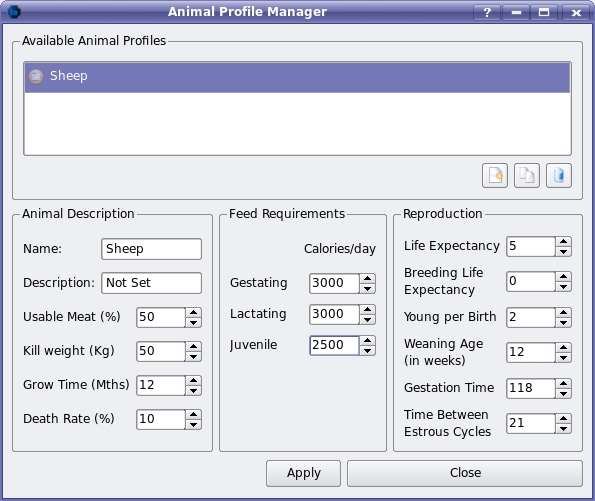
\includegraphics[scale=.39]{./images/animalManager.jpg}
    % animalManager.jpg: 683x452 pixel, 762dpi, 2.28x1.51 cm, bb=0 0 65 43
 \label{fig:animalManager} \caption{Animal Manager Form}
\end{figure}


  \begin{enumerate}
    \item \textbf{Animal Description}
      \begin{enumerate}
        \item \textit{\textbf{Name}}
        \item  \textit{\textbf{Notes}}
        \item  \textit\textbf{{Food Value}} - the number
of calories in one kilogram of meat from the animal.
        \item  \textit{\textbf{Usable Meat}} - the percentage of the animal's
live weight that is usable as food.
        \item  \textit{\textbf{Kill Weight}} - This is the live weight of the
animals at the time of slaughter.
        \item  \textit{\textbf{Grow Time}} - The length of time from birth to
slaughter weight.  This is quite important for estimating the herd size. The
longer it takes an animal to reach slaughter weight from birth, the higher the
number of animals alive at any given time.
        \item  \textit{\textbf{Death Rate}} - LandUse Analyst accommodates for
birthing deaths only. However, you can adjust the death
rate setting to indicate the average survival rate of births. This is important
for determining herd size, as it affects the number of mothers needed to sustain
the production levels required by the settlement. 
      \end{enumerate}

    \item \textbf{Reproduction}
      \begin{enumerate}
        \item  \textit{\textbf{Sexual Maturity}} - the age, in
months, at which the females become sexually mature
        \item  \textit\textbf{{Breeding Life}} - how long a female
can be expected to breed reliably.
        \item  \textit{\textbf{Young per Birth}}
        \item  \textit{\textbf{Weaning Age}} - The age of the babies, in weeks,
at which they stop feeding from their mother. It is assumed by LandUse Analyst
that mothers will become pregnant after one oestrous cycle following weaning. 
        \item  \textit{\textbf{Gestation Time}} -The number of days for
gestation. 
        \item  \textit{\textbf{Oestrous Cycle}} - The number of days in the
animal's oestrous cycle
      \end{enumerate}

    \item \textbf{Feed Requirements}
      \begin{enumerate}
        \item  \textit{\textbf{Gestating}} - calories required per
day for a female during gestation.
        \item  \textit{\textbf{Lactating}} - calories required per
day for a female while lactating.
        \item  \textit{\textbf{Juveniles}} - calories required
\textit{on average} for a juvenile.  Although future versions of Landuse Analyst
will incorporate the rise in feed requirements as juveniles grow from weanlings
to slaughter weight, at this early stage of development an average must be used.
      \end{enumerate}
  \end{enumerate}

  \subsection{Animal Model Parameters}
To define different parameters (see Fig. \ref{fig:animalParameters}) for the
same animal, follow the same procedure used for defining multiple animals with
the same name. Having multiple parameters can be useful for setting up different
scenarios, such as drought years, disease, catastrophic events, etc. Eventually,
Landuse Analyst will have the ability to model over time, and will have these
types of scenarios incorporated into the software.

\begin{figure}[htbp]
    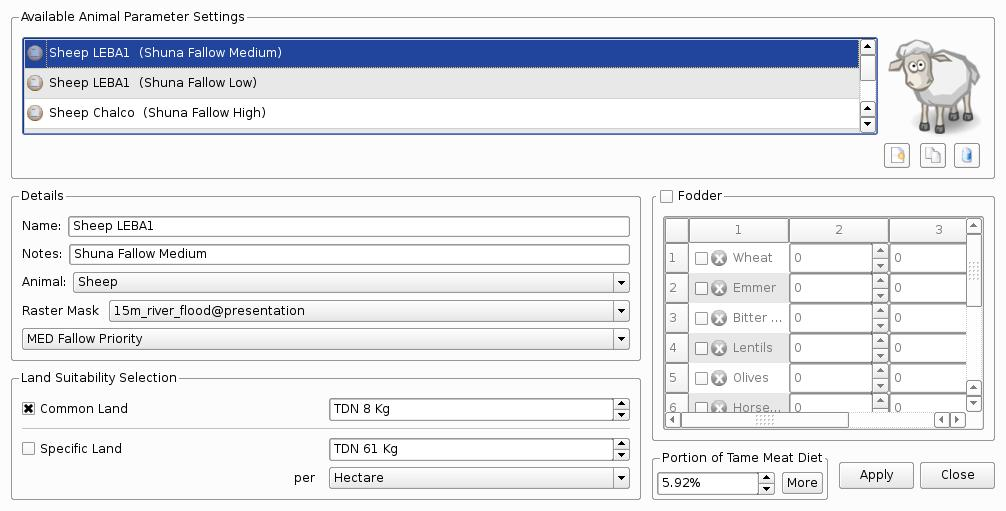
\includegraphics[scale=.23]{./images/animalParameters.jpg}
    % animalParameters.jpg: 1006x511 pixel, 762dpi, 3.35x1.70 cm, bb=0 0 95 48
  \caption{\label{fig:animalParameters}Animal Parameters Form}
\end{figure}

  \begin{enumerate}
    \item \textbf{Details}
      \begin{enumerate}
        \item \textit{\textbf{Name}}
        \item \textit{\textbf{Notes}} 
        \item \textit{\textbf{Animal}} -It is very important to select which
animal your parameter settings are for. Once you select the animal it appose to,
simply click Apply, and it will then be properly allocated, and will show up in
the dropdown list for that animal in the table on the top. 
        \item \textit{\textbf{Raster Mask}} - Select the raster mask file that
will be used to identify suitable land for this animal to graze.  Note that this
field is not needed if common land is being grazed.
        \item \textit{\textbf{Fallow Priority}} - If the animal grazes fallow,,
this is simply a way to give preferential access to fallow land to certain
animals.  There is no minimum or maximum number of animals per priority level,
so all animals could be set to High Priority, or all but one to Medium and one
to Low.  It is also acceptable to only allow one animal access to the fallow,
which can again be at any priority level.  (i.e. all animals can be set to not
graze fallow, and even if just one of them is set to low priority, it will get
access to all of the available fallow land)
      \end{enumerate}
    \item \textbf{Land Suitability Selection}
      \begin{enumerate}
        \item \textit{\textbf{Common Land}} -Sometimes land is suitable for
grazing by more than one type of animal. LandUse Analyst allows you to designate
one suitability mask as common grazing land. Note that you can specify an animal
to use both common land and specific land at the same time. If this is the case,
equal preference is given to all animals grazing the common land. This is not
always ideal, as it may have been the case that some animals were given
preference to the common land if the other suitable land was further away than
the other animals using it\footnote{A workaround for this problem is that
LandUse Analyst produces classified maps of the land being used, so if it is the
case that you find one animal being forced to travel much further than others,
you can simply change settings to balance this. This can be accomplished by
removing the other animals one at a time from using the common grazing land. It
may be the case, however, that there is no ideal solution, and that they simply
had to travel the extra distance!}.
        \item \textit{\textbf{Specific Land}} -Sometimes you may want to specify
that land is suitable for grazing by only one type of animal. LandUse Analyst
allows you to designate a land suitability mask as being unique to that animal.
Note that you can specify an animal to use both common land and specific land at
the same time. For more detailed information on this, see the help section on
Animal Common Land.   Note that the other setting in this section is for the TDN
(in Kg) per land area unit available for grazing animals per year.
          \begin{enumerate}
            \item \textit{\textbf{TDN}} - The TDN (in Kg) per land area unit
available for grazing animals per year.
            \item \textit{\textbf{Area Units}}
          \end{enumerate}
      \end{enumerate}
  \begin{enumerate}
    \item \textbf{Fodder} - If your settlement fed the animal fodder, check off
the Fodder section to enable the Fodder options to be accessible. 
      \begin{enumerate}
        \item \textit{\textbf{Crop}} - All of the crops being grown by the
settlement are in this list.  If our animal which you are setting the parameters
for are utilising this crop's fodder, either directly by eating the grain, or
indirectly by eating it's straw and chaff, simply indicate the percent of it's
diet that is being provided by each.
        \item \textit{\textbf{Grain}} - If your animal is fed grain harvested
from a crop, indicate the percentage of the animals diet being supplied by it
is. 
        \item \textit{\textbf{Straw \& Chaff}} - If your animal is fed straw or
chaff left over after harvesting a crop, indicate what percentage of the animals
diet being supplied by this by-product. 
      \end{enumerate}
  \end{enumerate}
    \item \textit{\textbf{Percent of Diet}}
\end{enumerate}

\begin{figure}[htbp]
    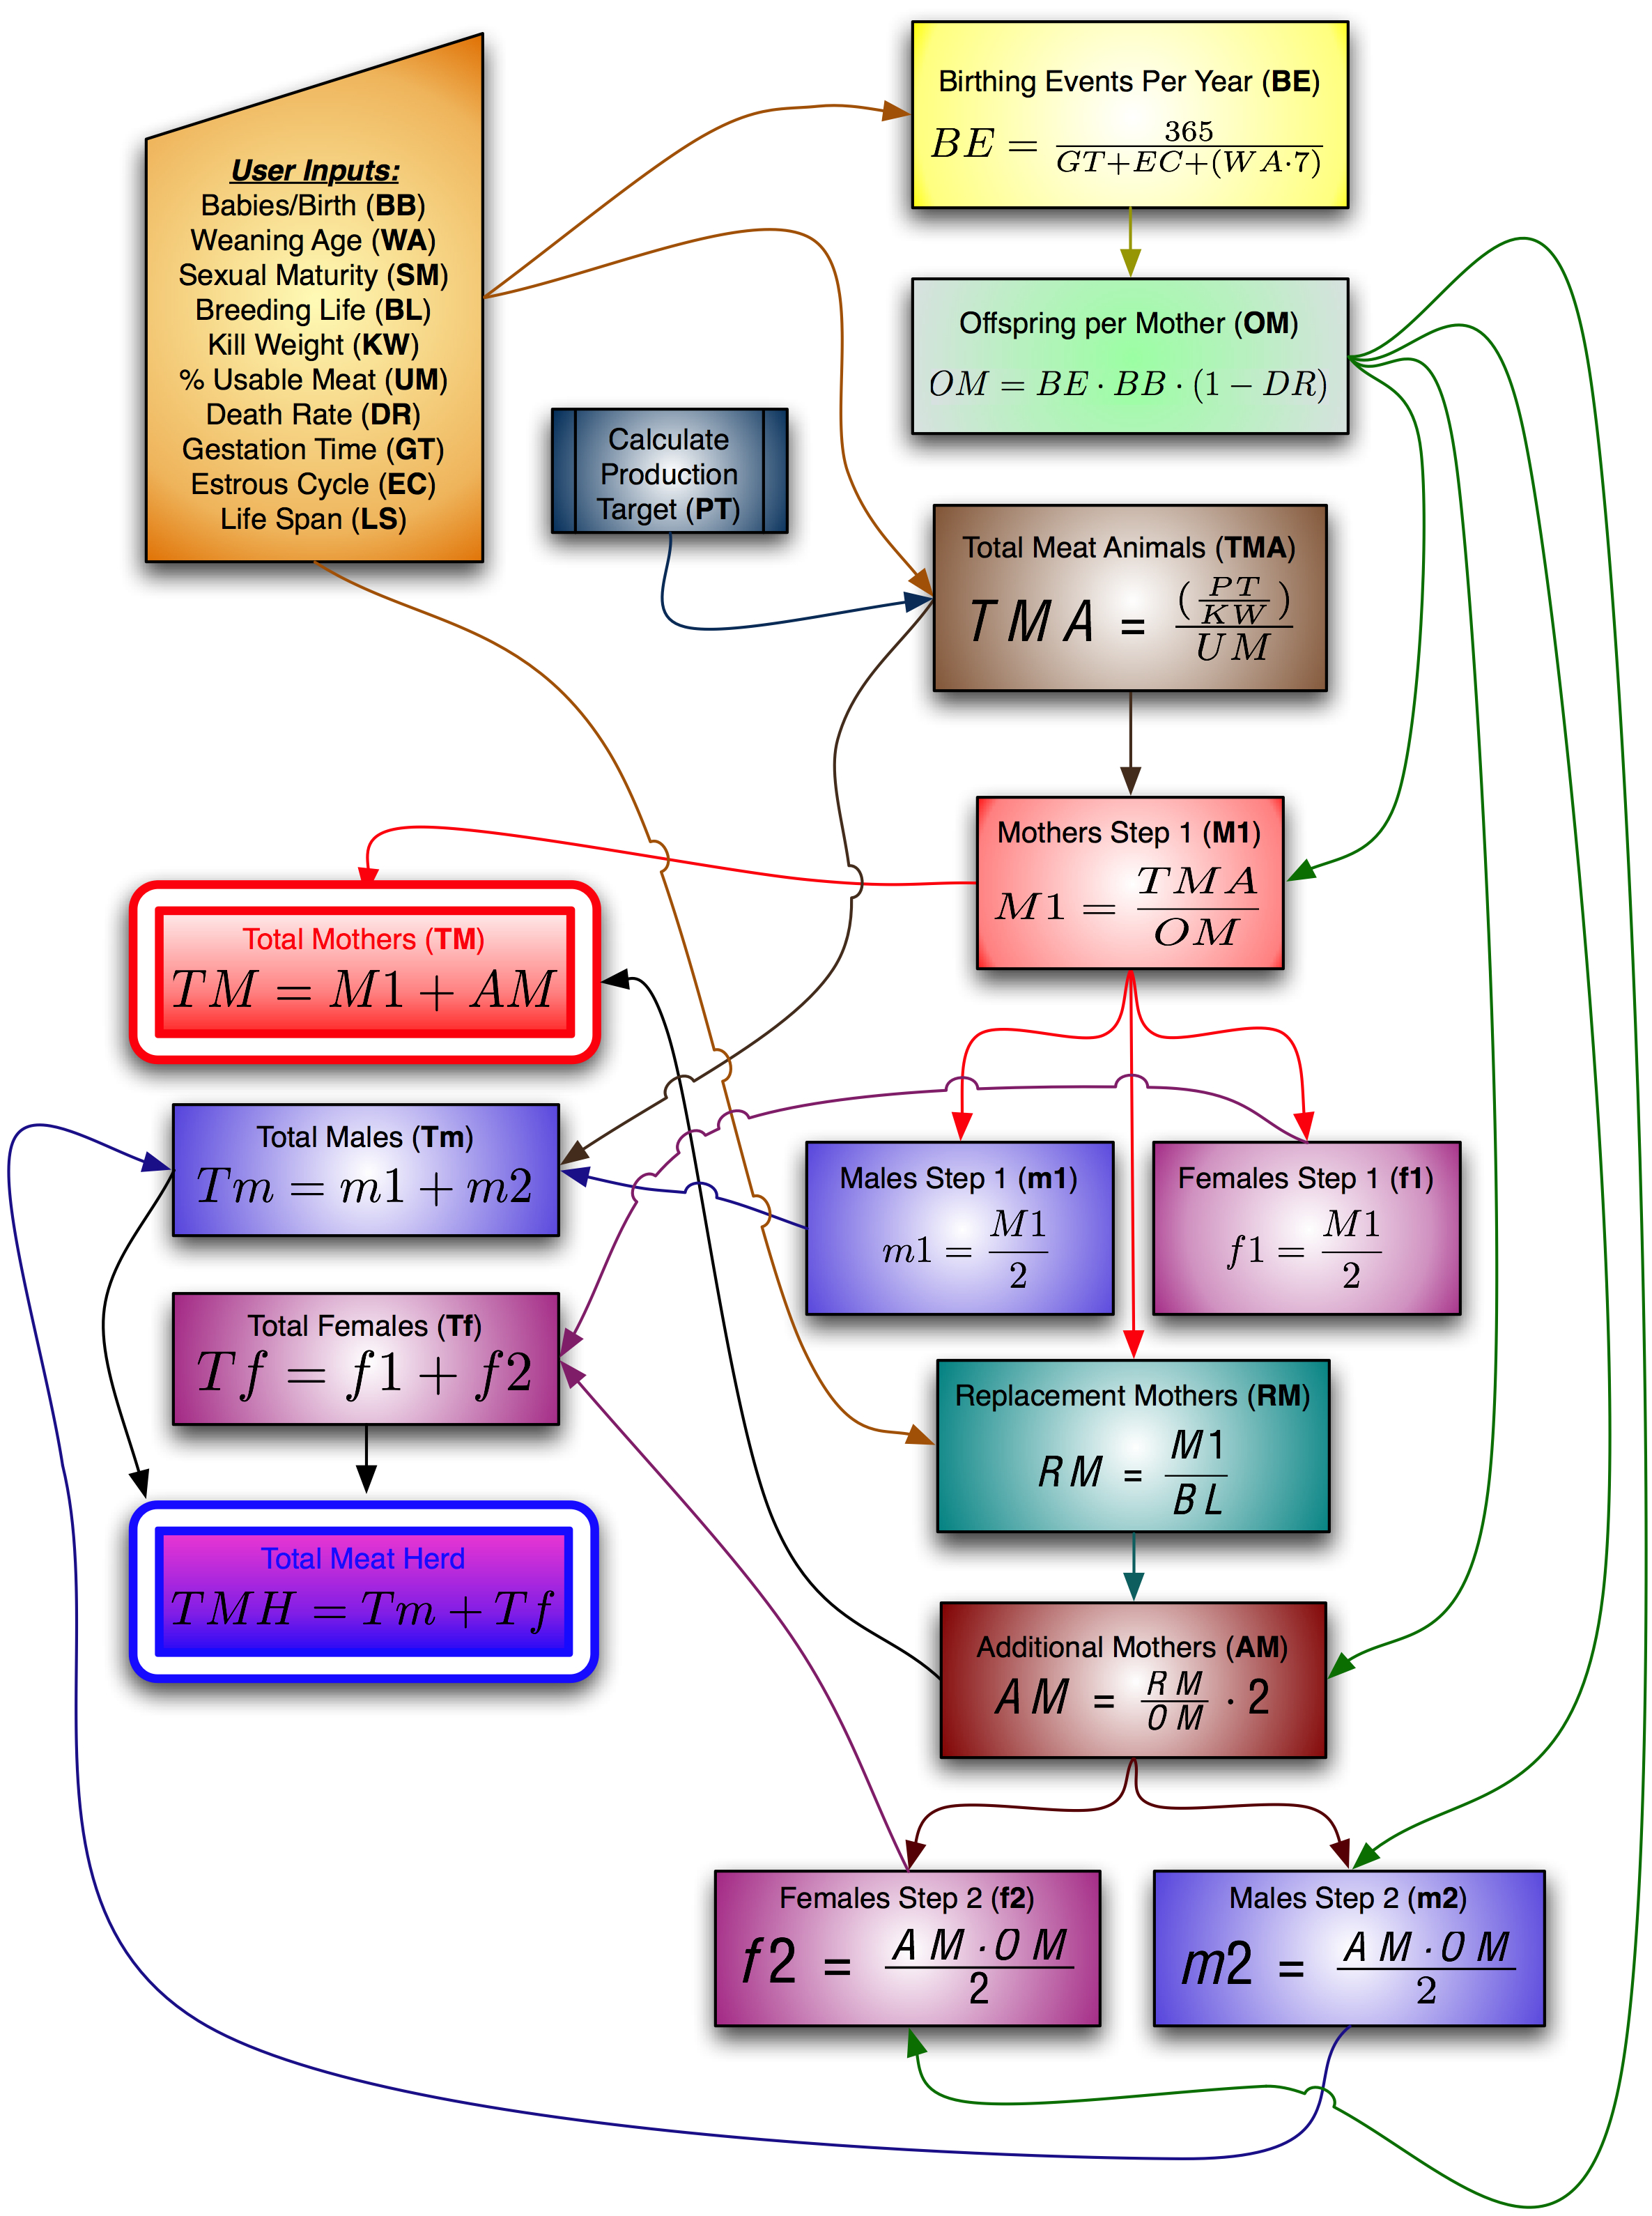
\includegraphics[scale=.4]{./images/animalHerdSize.jpg}
    % animalHerdSize.jpg: 2371x3180 pixel, 300dpi, 20.07x26.92 cm, bb=0 0 569
763
    \caption[Animal Herd Size Calculation]{\label{fig:herdSize}\textit{Animal
Herd Size Calculation - This diagram assumes that the production target has
already been worked out.  Units for input variables are: \textbf{WA}-days,
\textbf{SM}-months, \textbf{BL}-years, \textbf{KW}-kg, \textbf{DR}-percentage,
\textbf{GT}-days, \textbf{EC}-days, \textbf{LS}-years, \textbf{PT}-kg.}}
\end{figure}

\section{Herd Size Calculation}
The size of the herd required to sustain a particular amount of meat for a
population is crucial for determining an area target for each type of animal
raised.  An algorithm generic enough to make this calculation for any animal
that has been defined in Landuse Analyst was created. By taking the Production
Target and several user inputs, the total number of adult females (Mothers) and
animals being raised for meat (Meat Animals) can be approximated. This process
is outlined in Fig. \ref{fig:herdSize}.

\section{Catchment creation methods} 

When searching for land that meets the area targets, LA starts at
the coordinates of the settlement and moves outward to a point where the land
contained within equals the area target.  LA implements three
different methods for searching outwards from the settlement.  The key
difference between the three methods is the way in which a cost-surface gets
generated, which we will now examine.  All three methods currently used by LA
require a \textbf{D}igital \textbf{E}levation \textbf{M}odel (DEM) to generate
the cost surfaces.


  \subsubsection{Euclidean} \label{subsection:Euclidean} 
  
  This method ignores all topographic features of the landscape when moving
  outwards from the site.  Essentially we are drawing circles around the site,
  with the site right in the middle.  Drawbacks to using this method exist.
  Whilst moving across a landscape, people are affected by slope, rivers,
  landcover, etc.  Circles are just convenient when there is no easy way to
  calculate with an alternative method.  The primary reason for its inclusion
  as a catchment area creation method in LA is to provide the user
  with the option of seeing the difference between this rather simplistic
  approach and the other two methods.

  \subsubsection{Path Distance}\index{Path Distance}
  
  Path Distance is a cost surface creation method that looks at elevation data
  from a DEM and calculates distance from the site taking into account the
  extra distances travelled going up or down slopes.

  \subsubsection{Walking Time}\index{Walking Time}
  
  Walking Time is likely going to be the primary choice of the three methods of
  creating catchment areas in LA.  The cost surface that is
  generated for this method (see Fig. \ref{fig:rwalk}) uses a DEM to calculate
  how long it would take to walk from a starting point (the site, or ZERO on
  the cost surface) to all points on the DEM within a five hour walk ($18,000$
  seconds). Five hours is simply the time used for this case
  study\footnote{This number is currently hard coded. Future versions will
  allow the user to edit this value.} This creates a cost surface with values
  from $0$ to $18,000$ (See Fig. \ref{fig:rwalk}).  

%\setkeys{Gin}{width=1\textwidth}
\begin{figure}[htbp] \centering
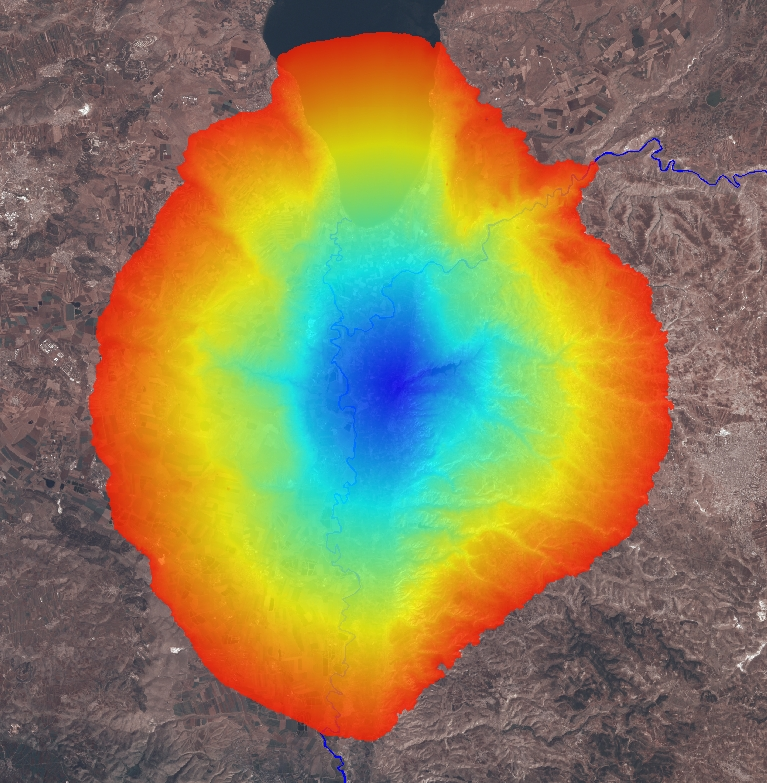
\includegraphics[scale=0.29]{./images/rwalkShuna.jpg}
   %caption of the figure
   \caption{LA generated this surface using the GRASS module r.walk.}
   \label{fig:rwalk} \end{figure}

\section{Land suitability raster masks} 

The land suitability masks must be binary rasters, meaning that the cells of
the raster file only contain 0 or 1 (NULL values are currently not supported).
The land that is deemed suitable for use should be set to a value of 1, and the
rest of the land is set to 0.  This binary raster  can then be multiplied by a
selection layer (as created by either Walking Distance, Path Distance,
or Euclidean methods).  This selection layer (also a binary raster) grows in
size until enough area is
found within it's bounds - identifying the land to be analysed.

In the current version, the software gives the option using three different
methods for landuse classification.  They are: 

\begin{enumerate} 

\item  Use only the user supplied classification map (a binary mask) 

\item  Use minimum and maximum slope values to create a classification map
which will be used exclusively.  This can be done for common crop land and
common grazing land independently.  For example, the user might stipulate
$0^\circ \leq m \leq 9^\circ$ for crops and $9^\circ < m \leq 15^\circ$ for
grazing land, where $m=slope$.  

\item  Using a combination of the two classification maps.  Slope can be chosen
to either add to or subtract from the user supplied map, or alternatively, the
user supplied map can either add to or subtract from the slope map.  This
combination of the two can be very useful if, for example, a user wishes to use
a soil classification map as the primary indication of landuse suitability, but
refine that map by taking out the land they consider too steep for use.  In
this case the program generated slope masks would be subtracted from the user
supplied (soil) classification map.  

\end{enumerate}

  \begin{figure}[htbp] %Location
  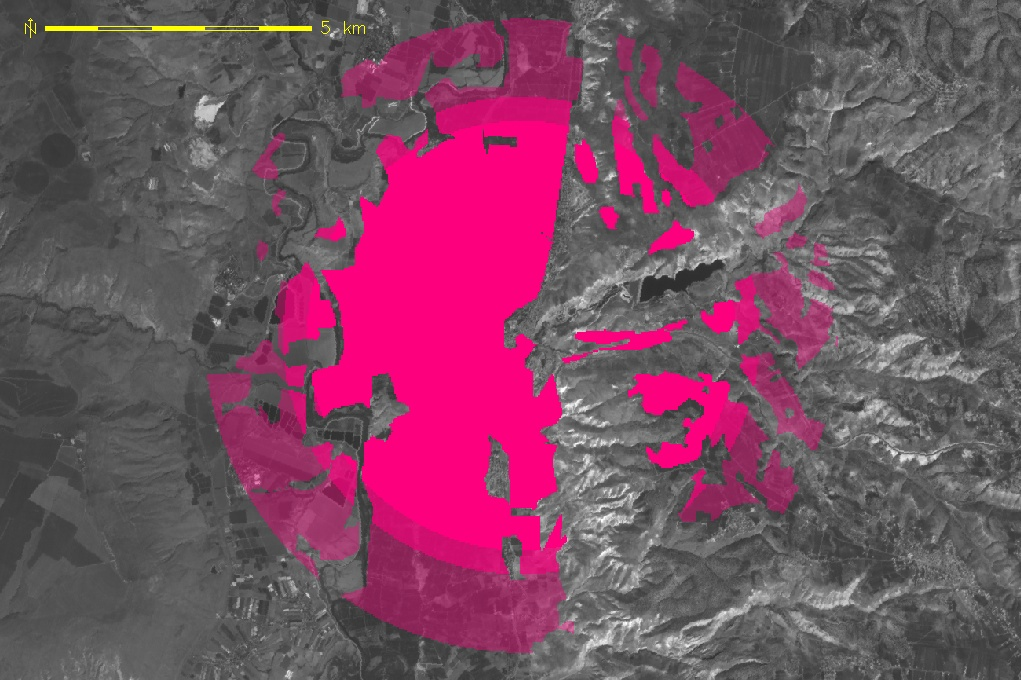
\includegraphics[scale=0.225]{./images/landcatchment.jpg}
   % img42.jpg: 800x600 pixel, 72dpi, 28.22x21.17 cm, bb=0 0 800 600
   \label{fig:landCatchment} \caption{Results which identified the suitable
         land surrounding Shuna using Euclidean method.
   The different shades represent different settlement populations.}
   \end{figure}

\section{Finding the land} 

In order to find the suitable land required
to produce enough food to sustain the settlement that is in closest proximity, 
a conditional loop is used which defines the outer extent of the catchment
area, 
and then calculates the area of suitable land contained within it.  This process
is identical for all
analysis methods.  The earliest versions of LA started at the
closest point to the site that could potentially solve the problem
\footnote{The closest point, or minimum radius, is a perfect circle equal in
area to the target.}, and then moved steadily outwards until the area target
was found.  The amount to move outward in each step was a value provided by the
user, and might have been a value like 30 (which in the case of walking
distance meant 30 seconds, on  a cost surface of 20,000.  This would mean that
potentially, there would have to be $\frac{20,000}{30}$ or nearly 7000
iterations!)
The basic steps involved were:

   \begin{enumerate} 
   
   \item  Set the initial boundary to start the analysis
   
   \item  Calculate the area of suitable land found within this boundary 
   
   \item If the area of land required has been satisfied, write the results to a
new
   file for that item and exit the loop 
   
   \item  Increase the value of the analysis boundary 
   
   \item  Repeat the loop (starting at Step 2)
   
   \end{enumerate}

This method proved extremely time consuming;  If even 3,500 loops, which is
about half of the cost surface map, was required, and each loop took as little
as 45 seconds, the computation time was nearly 44 hours.   To increase the
efficiency, a modified binary search is now used.  This involved a somewhat
different approach.  Instead of using a step amount, a percentage is used.
This percentage value is called the \textit{Precision}. 
The area of land deemed as equalling the current area target gets changed into
a range $\pm$ the precision value multiplied by the target area. 
If a value of $5\%$ is entered, and the area
target is 100 hectares, LA accepts $100 \pm(\frac{100 \cdot
5\%}{2})$ (which is $97.5$ to $102.5$ hectares) as the target area.  The loop
uses three terms, $CurrentMidValue$ $FirstValue$ and $LastValue$ At the
beginning of the process, $FirstValue=0$ and $LastValue=18,000$ which coincides
with the full extent of the cost surface.  $CurrentMidValue$ is calculated
within the loop.  The loop works like this:

  \begin{enumerate} 
  
  \item Set the analysis boundary: $CurrentMidValue=\frac{FirstValue +
  LastValue}{2}$.  
  
  \item Calculate the area of suitable land found within the boundary whose
  outermost boundary is $CurrentMidValue$ 
  
  \item If the contained area falls within the target range, write the results
  to a new file and exit the loop 
  
  \item If the contained area is more than the maximum value in the target
  range, set a halfway between $FirstValue$ and $CurrentMidValue$. This is done
  by making $LastValue=CurrentMidValue$ and then returning back to step number
  one.  (Note $FirstValue$ remains unchanged.) 
  
  \item If the contained area is less than the minimum value in the target
  range, set a halfway between $LastValue$ and $CurrentMidValue$. This is done
  by making $FirstValue=CurrentMidValue$ and then returning back to step number
  one.  (Note $LastValue$ remains unchanged.) 
  
  \end{enumerate}

By using this method, the \textit{maximum} number of steps in the loop is 17.
This method of searching for the area targets made a huge difference in Landuse
Analyst's speed\footnote{ a typical 'run' on a decent computer system is
$\approx$ 2 to 3 minutes now, compared to up to two weeks using the original
method.}, allowing users to now examine many different variations of an entire
model quickly and easily even on an average computer system.  The resultant
maps clearly show which land was likely to have been used, and for what purpose
it was being used for\ref{fig:caseStudy}
 
  \begin{figure}[htbp] %Location
  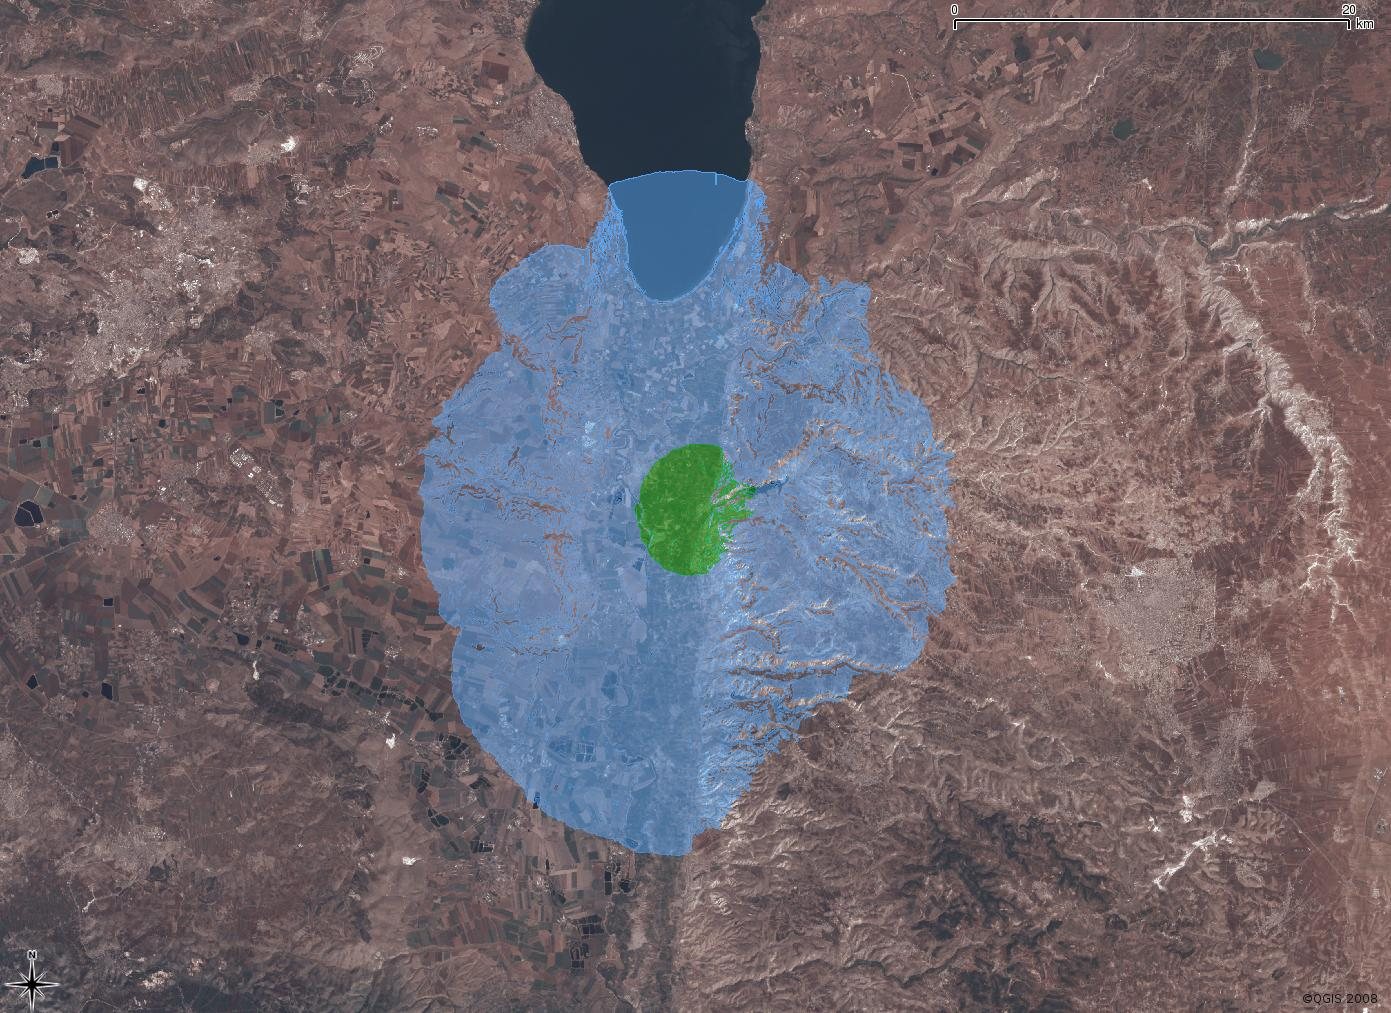
\includegraphics[scale=0.225]{./images/LEB130007030FallowSlope.jpg}
  \label{fig:caseStudy} \caption{Case Study: Shuna  Population 3000, EB1a. 
Green is for growing crops, blue for grazing.  Walking Time was used to create
the cost surface.}
  \end{figure}

\section{Future development} \label{FuturePlans} 

LA is still in the early stages of its development and many
improvements to usability and application capabilities are planned. That said,
the application is already capable of producing useful results (though more
testing is still needed) in a more flexible, user friendly and efficient manner
than the original BASH prototype.

There are many routes that LA can take from this point with
respect to it's future development; it can continue on as a standalone
application, or turn into a plugin for another application like openModeller or
QGIS.  Before these decisions are made, however, the features in the current
version must be finalised and implemented.  Some features which are currently
in the planning phase are network analysis  for inter-site relationships,
experiment settings, where the model can be set to run a given number of times
using different input variables, and report generation complete with graphs and
maps. 

The network analysis feature will look at all contemporaneous sites in a given
area, and examine production potential.  If a site can potentially produce
excess meat, but falls short in cropland, it will look to neighboring sites to
see if they can make up the difference.  If there is a potential for trade or
supplementation, the most efficient walking routes can then be found using
r.drain on a cost surface generated with r.walk.  This could potentially show
the likely pathways between sites, as well as how intensively used they might
have been.  Taking this further, one might look for places where these routes
merge, or cross, which might be an indicator for a potential archaeological
site which has yet to be discovered.

The current version of LA requires that every scenario be modelled
manually and separately.  For example, one might wish to look at how adjusting
the yield of crops would affect the land requirements to simulate drought
years.  One might also want to compare the results of different dietary
proportions of meat content to plant content.  With the experiment module, it
will be possible to have the software automatically cycle through all of these
different scenarios automatically.

Drawing much on the work done in openModeller, there is also the hope that it
will be possible to have LA compile presentation quality reports,
complete with spreadsheets and graphs.  This will be a great time saving
feature.  In addition, this will provide a consistency that will make it much
easier to systematically compare results with other users.

Anyone interested in knowing more about this project, or better yet, in
contributing to it, please don't hesitate in contacting us.


%etc.  \end{smallverbatim}


%if you want to cite please use:

% \cite{name:year} or \citep{name:year}

%.... revealed by \cite{herborg:2003} if it shall be in parentheses use
%\citep{herborg:2003}


%End of text.



\begin{footnotesize}
%\begin{thebibliography}{99}

%\bibitem[Herborg et~al. (2003) Herborg, Bentley, Clare, Rushton]{herborg:2003}
%L.M. Herborg, M.G. Bentley, A.S. Clare, S.P. Rushton (2003) \newblock The
%spread of the Chinese mitten crab (Eriocheir sinensis) in Europe; the
%predictive value of an historical data set.  \newblock {\em Hydrobiologia}
%503: 21-28.


%\end{thebibliography}
\end{footnotesize}


\address{Jason Jorgenson\\ University of Liverpool\\
\url{http://www.arkygeek.com} (under development)\\
\email{jjorgenson@gmail.com}}

\address{Tim Sutton\\ Centro de Referncia em Informao Ambiental, CRIA\\
\url{http://cria.org.br}\\
\email{timlinux@linfiniti.com}}

%%% Local Variables:
%%% mode: latex
%%% TeX-master: main_document.tex
%%% End: